% ft-excel-03-functions.tex

\documentclass[xcolor=dvipsnames]{beamer}
\usepackage{teachbeamer}

\title{Excel Functions}
\subtitle{MATH {\CourseNumber}, BCIT}

\author{\CourseName}

\date{October 1, 2018}

\begin{document}

\begin{frame}
  \titlepage
\end{frame}

\begin{frame}
  \frametitle{Excel Functions I}
  \begin{tabular}{|l|l|}\hline
    \textbf{Excel Function} & \textbf{Description}                                                                                             \\ \hline
    SUM            & Calculates the sum of a group of values                                                                 \\ \hline
    AVERAGE        & Calculates the mean of a group of values                                                                \\ \hline
    COUNT          & \specialcell[t]{Counts the number of cells in a range that\\contains numbers}                                             \\ \hline
    INT            & \specialcell[t]{Removes the decimal portion of a number\\leaving just the integer portion}                                \\ \hline
    ROUND          & \specialcell[t]{Rounds a number to a specified number of\\decimal places or digit positions}                              \\ \hline
  \end{tabular}
\end{frame}

\begin{frame}
  \frametitle{Excel Functions II}
  \begin{tabular}{|l|l|}\hline
    \textbf{Excel Function} & \textbf{Description}                                                                                             \\ \hline
    IF             & \specialcell[t]{Tests for a true or false condition and\\then returns one value or another}                               \\ \hline
    NOW            & Returns the system date and time                                                                        \\ \hline
    TODAY          & Returns the system date without the time                                                                \\ \hline
    SUMIF          & \specialcell[t]{Calculates a sum from a group of values\\but just of values that are included because\\a condition is met} \\ \hline
    COUNTIF        & \specialcell[t]{Counts the number of cells in a range\\that match a criteria}                                             \\ \hline
  \end{tabular}
\end{frame}

\begin{frame}
  \frametitle{Exercises}
have a look at \texttt{PHIL375grades.xls}. Answer the following questions.
  \begin{enumerate}
  \item<1-> How many essays were graded in total?
  \item<2-> Compare essay grades for the two different graders.
  \item<3-> What is the maximum and minimum score on the final exam?
  \item<4-> What is the average final grade for the course?
  \item<5-> How many students have a final grade in the 70-100\% range?
  \item<6-> How many students have a final grade in the 50-70\% range?
  \item<7-> How many students consistently score more than 80\% on essays?
  \end{enumerate}
\end{frame}

\begin{frame}
  \frametitle{PHIL 375 Grades Screen Shot 1}
  \begin{figure}[h]
    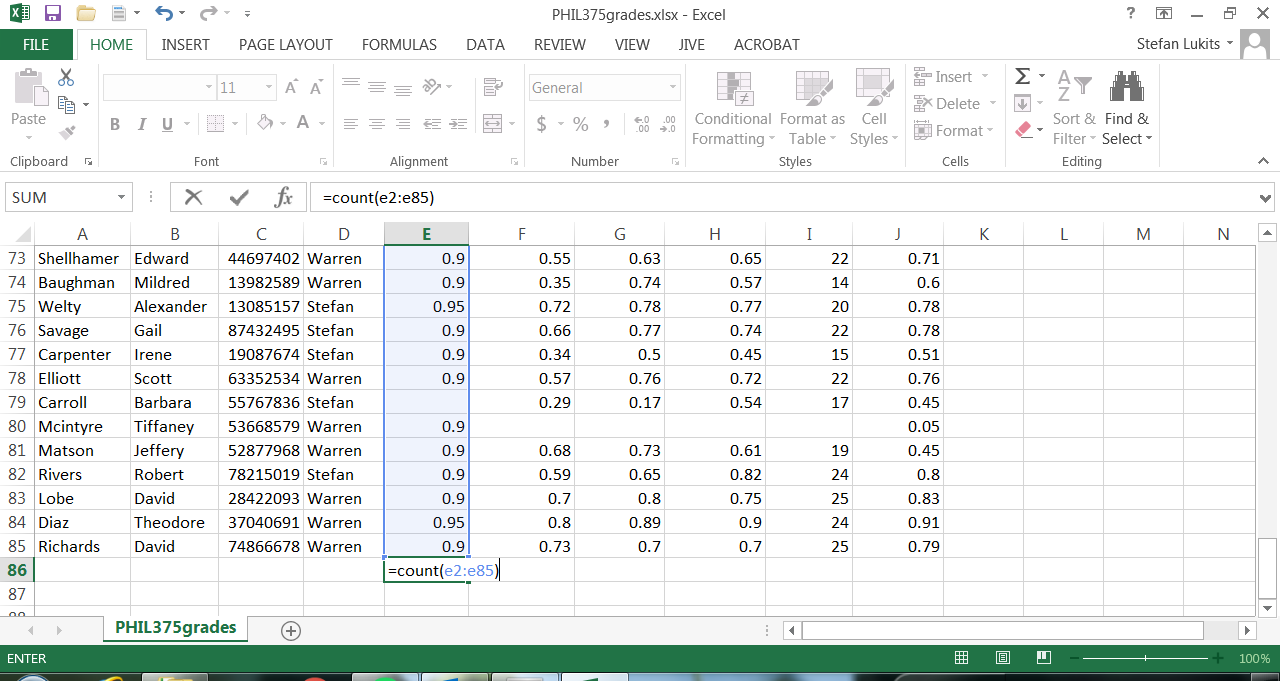
\includegraphics[scale=.42]{./e01.PNG}
  \end{figure}
\end{frame}

\begin{frame}
  \frametitle{PHIL 375 Grades Screen Shot 2}
  \begin{figure}[h]
    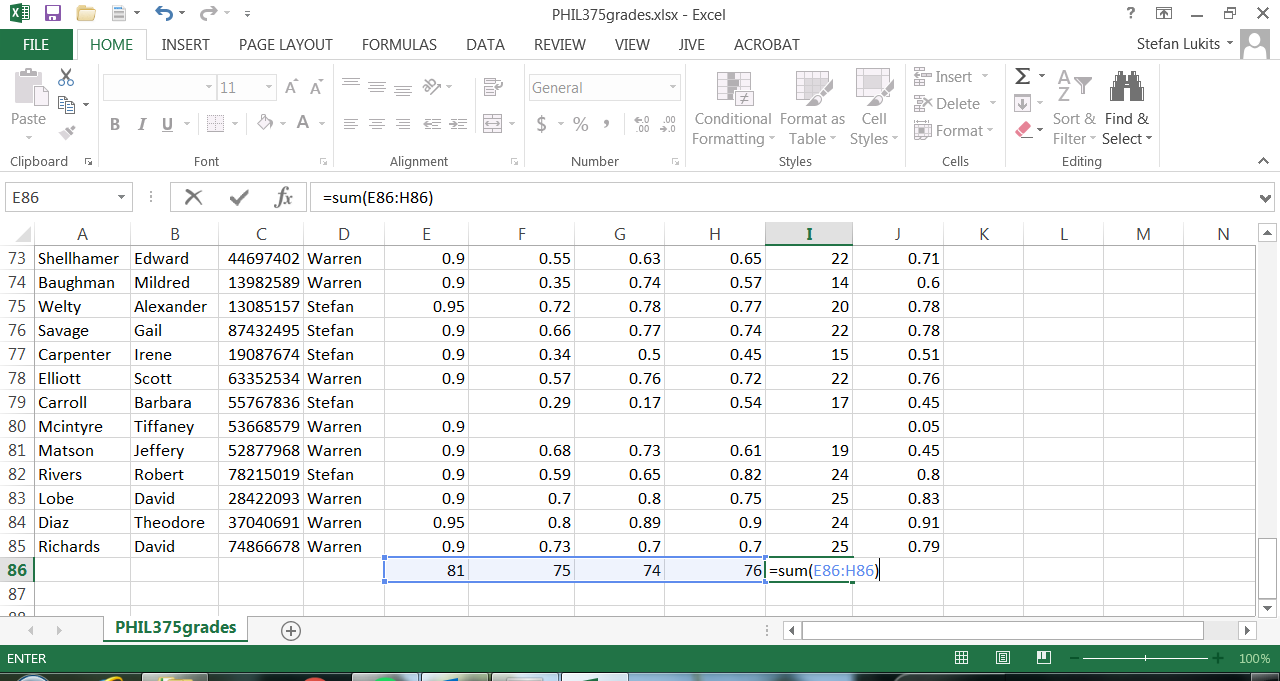
\includegraphics[scale=.42]{./e02.PNG}
  \end{figure}
\end{frame}

\begin{frame}
  \frametitle{PHIL 375 Grades Screen Shot 3}
  \begin{figure}[h]
    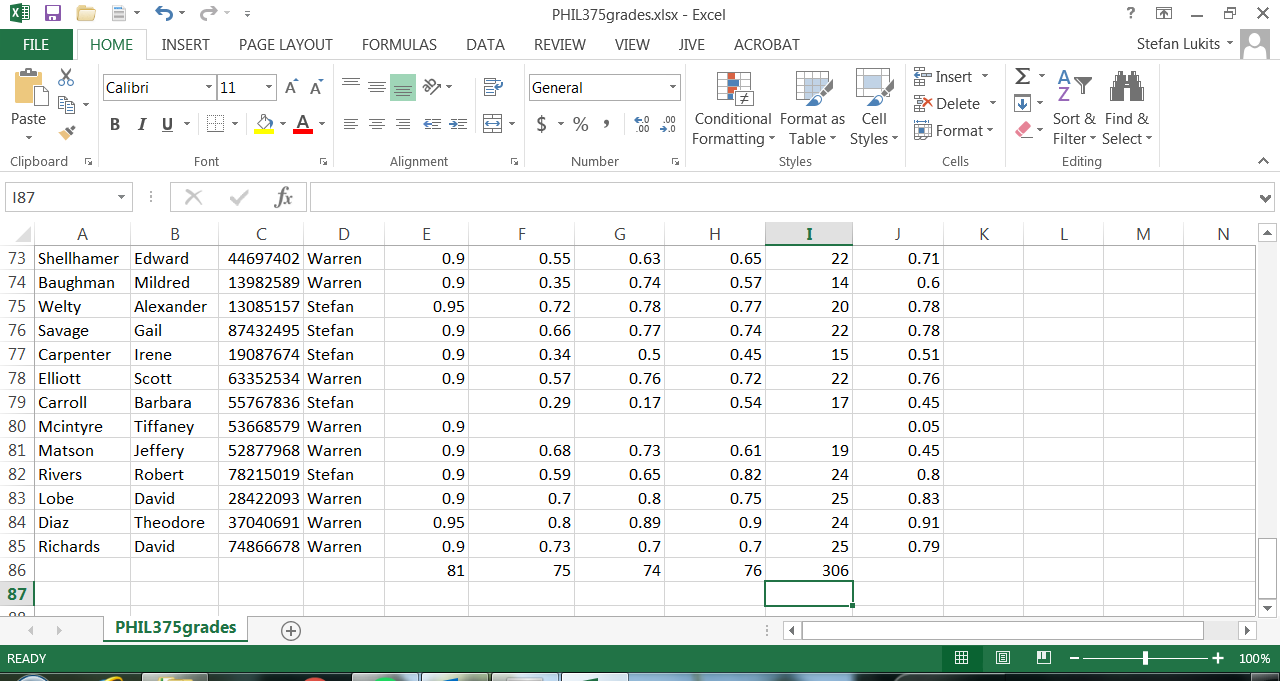
\includegraphics[scale=.42]{./e03.PNG}
  \end{figure}
\end{frame}

\begin{frame}
  \frametitle{PHIL 375 Grades Screen Shot 4}
  \begin{figure}[h]
    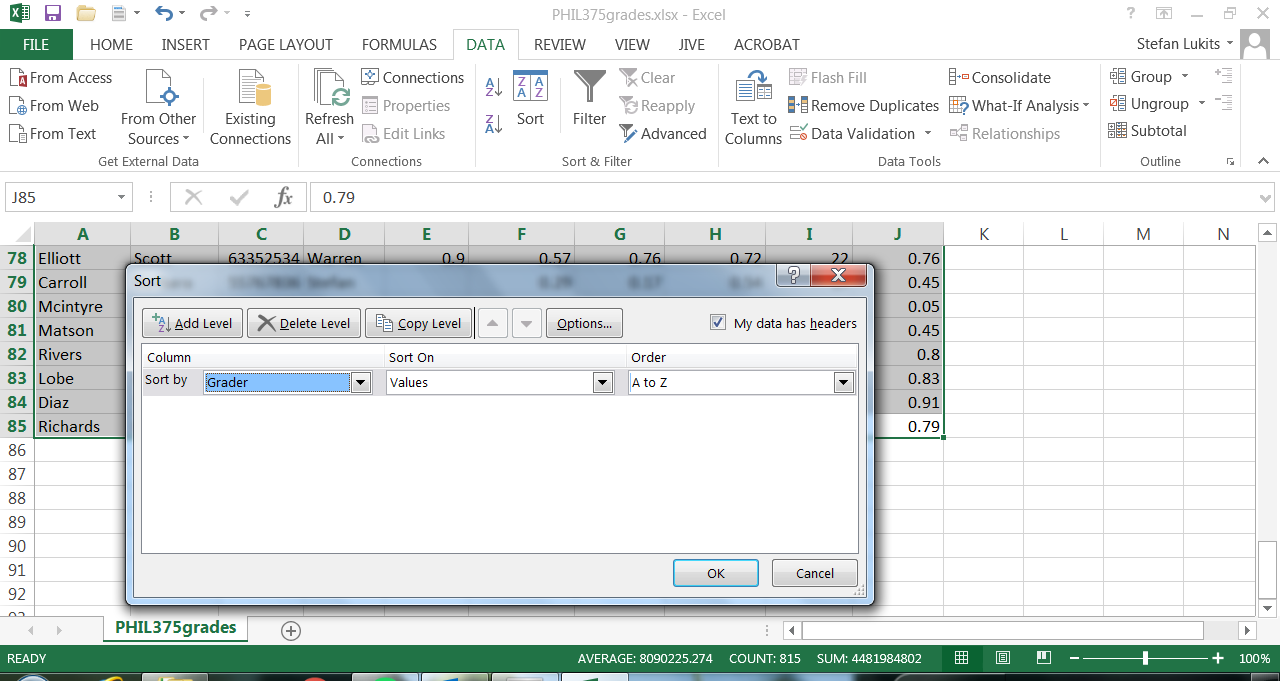
\includegraphics[scale=.42]{./e04.PNG}
  \end{figure}
\end{frame}

\begin{frame}
  \frametitle{PHIL 375 Grades Screen Shot 5}
  \begin{figure}[h]
    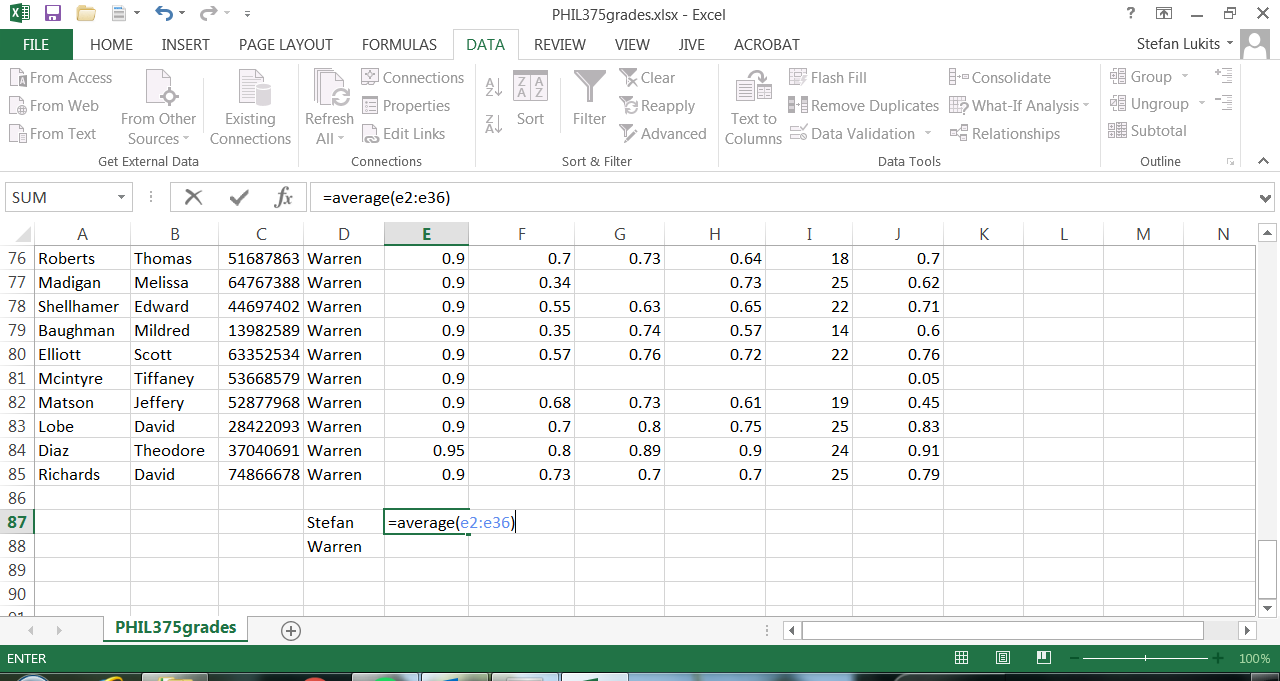
\includegraphics[scale=.42]{./e05.PNG}
  \end{figure}
\end{frame}

\begin{frame}
  \frametitle{PHIL 375 Grades Screen Shot 6}
  \begin{figure}[h]
    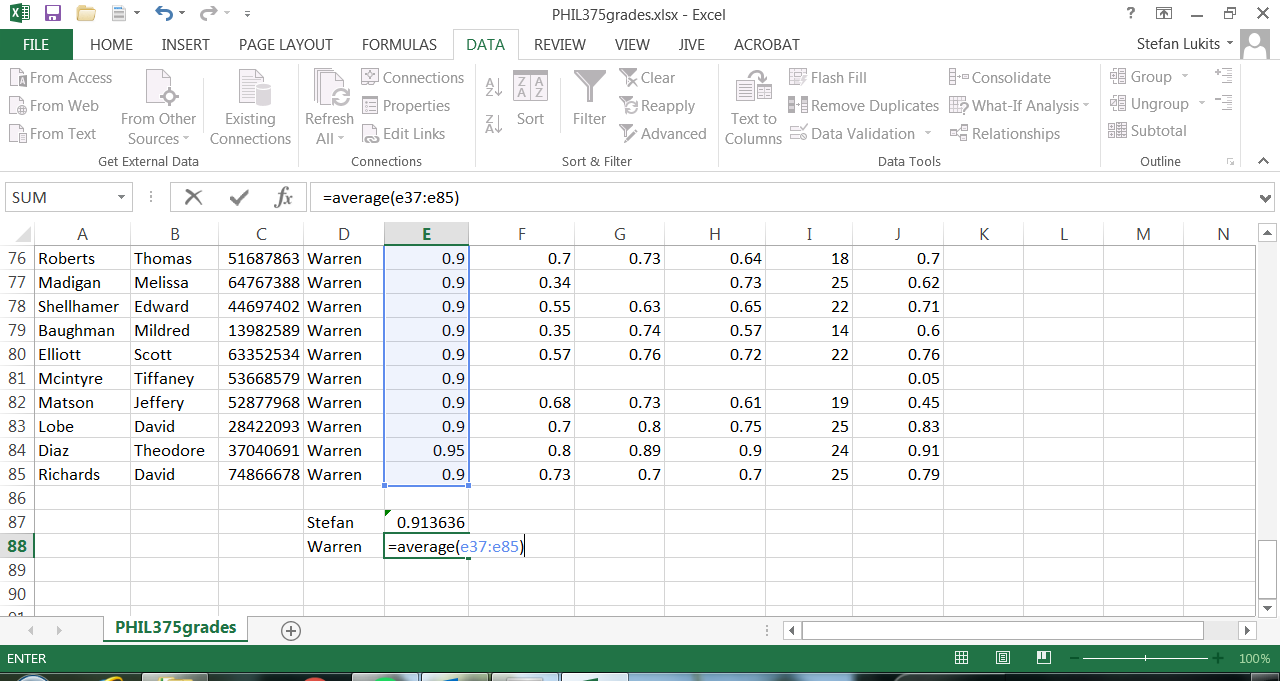
\includegraphics[scale=.42]{./e06.PNG}
  \end{figure}
\end{frame}

\begin{frame}
  \frametitle{PHIL 375 Grades Screen Shot 7}
  \begin{figure}[h]
    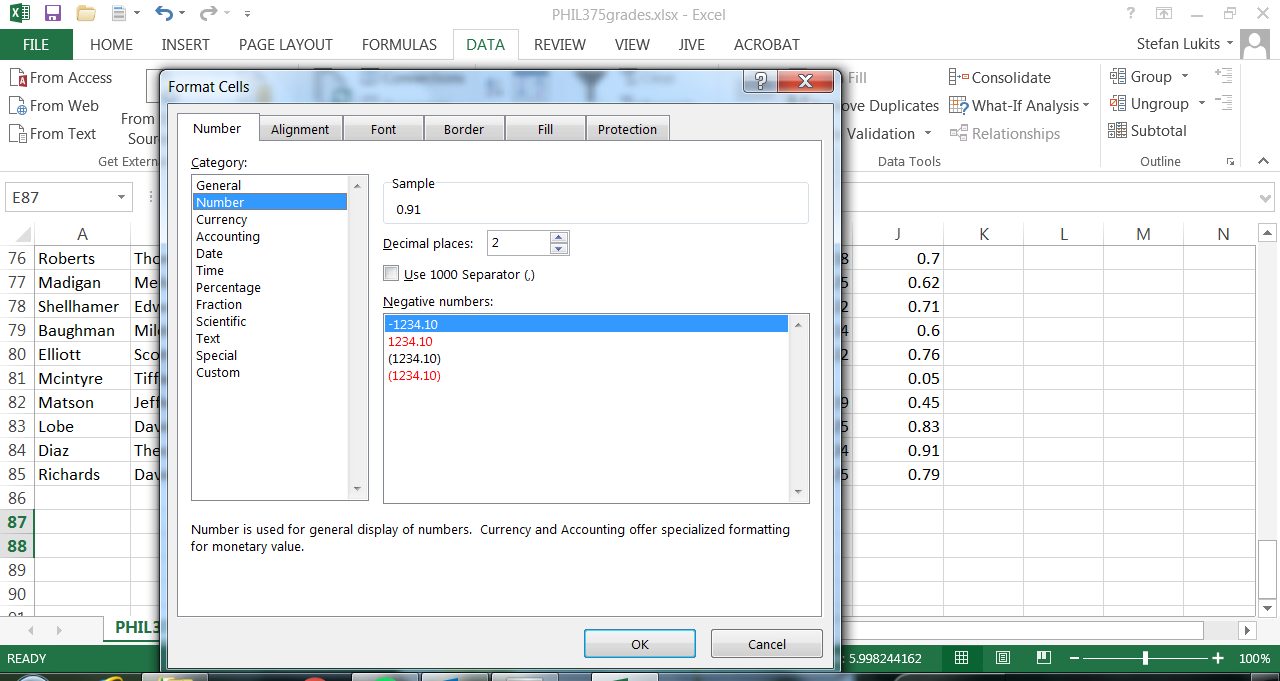
\includegraphics[scale=.42]{./e07.PNG}
  \end{figure}
\end{frame}

\begin{frame}
  \frametitle{PHIL 375 Grades Screen Shot 8}
  \begin{figure}[h]
    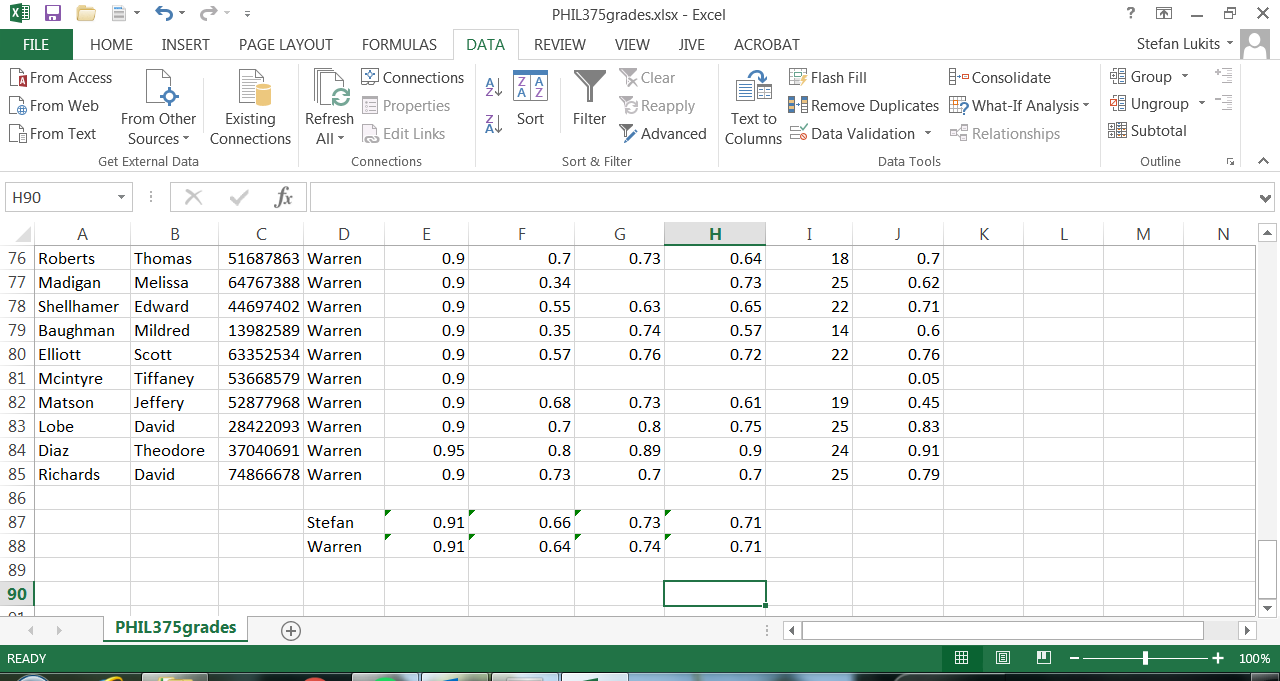
\includegraphics[scale=.42]{./e08.PNG}
  \end{figure}
\end{frame}

\begin{frame}
  \frametitle{PHIL 375 Grades Screen Shot 9}
  \begin{figure}[h]
    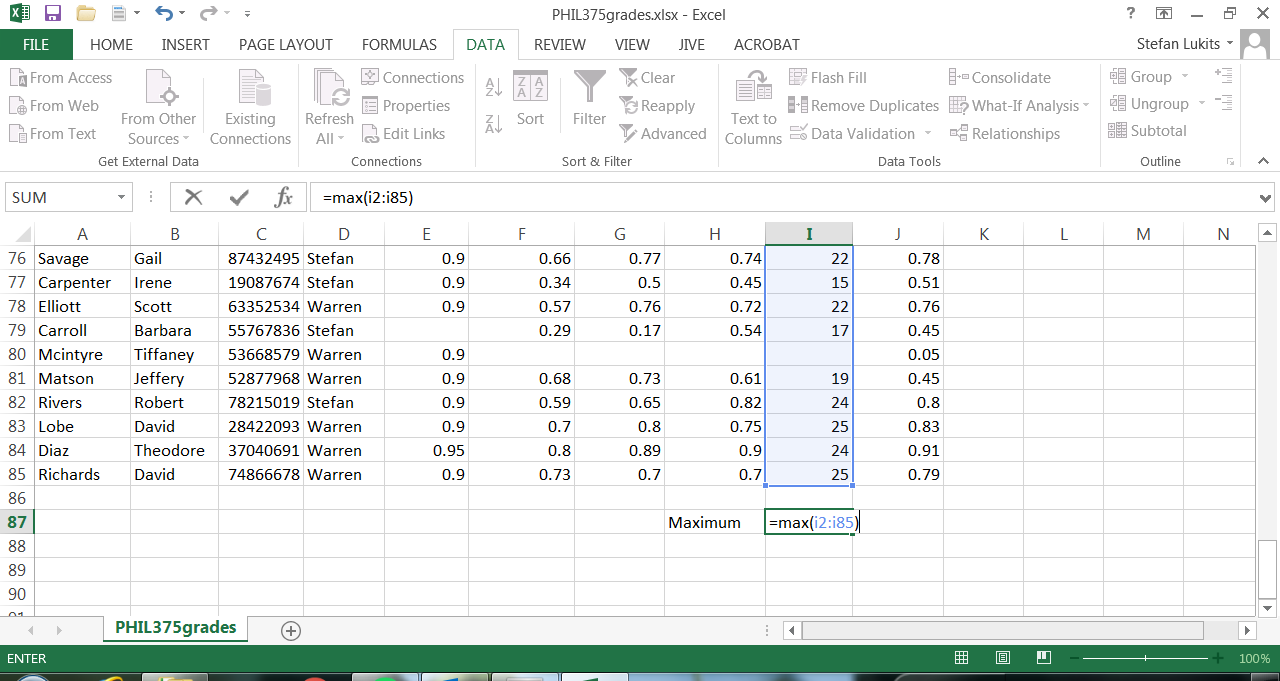
\includegraphics[scale=.42]{./e09.PNG}
  \end{figure}
\end{frame}

\begin{frame}
  \frametitle{PHIL 375 Grades Screen Shot 10}
  \begin{figure}[h]
    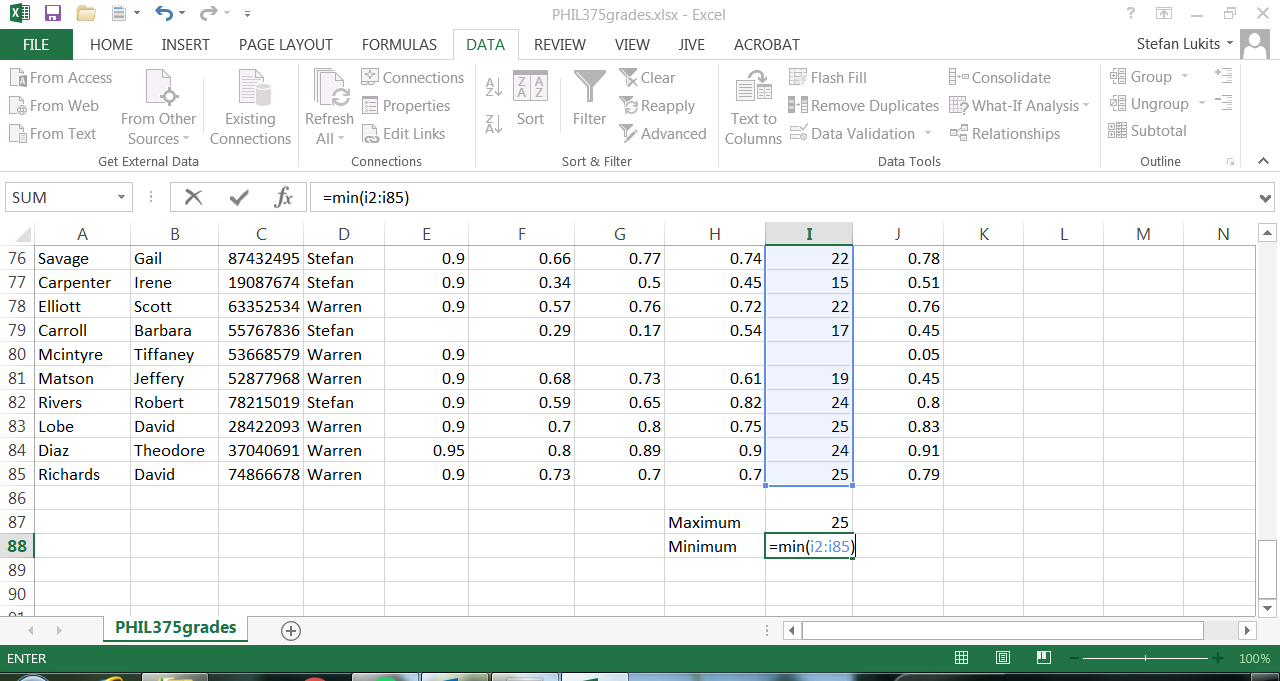
\includegraphics[scale=.42]{./e10.PNG}
  \end{figure}
\end{frame}

\begin{frame}
  \frametitle{PHIL 375 Grades Screen Shot 11}
  \begin{figure}[h]
    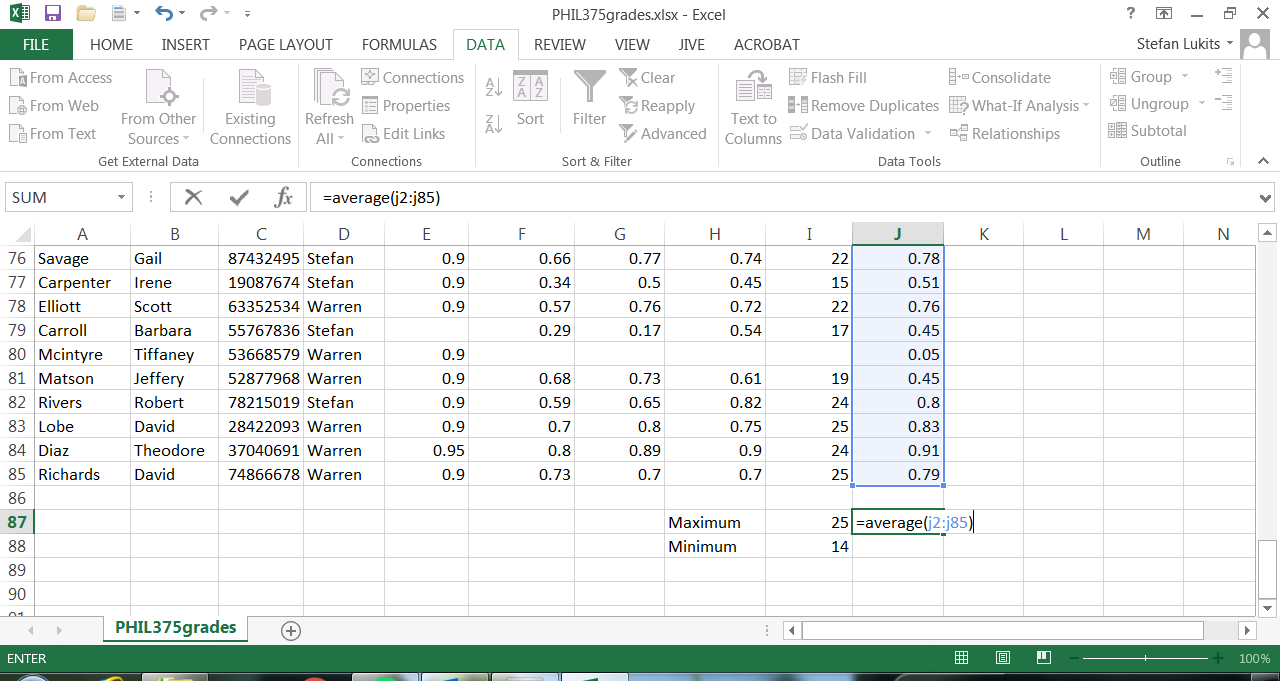
\includegraphics[scale=.42]{./e11.PNG}
  \end{figure}
\end{frame}

\begin{frame}
  \frametitle{PHIL 375 Grades Screen Shot 12}
  \begin{figure}[h]
    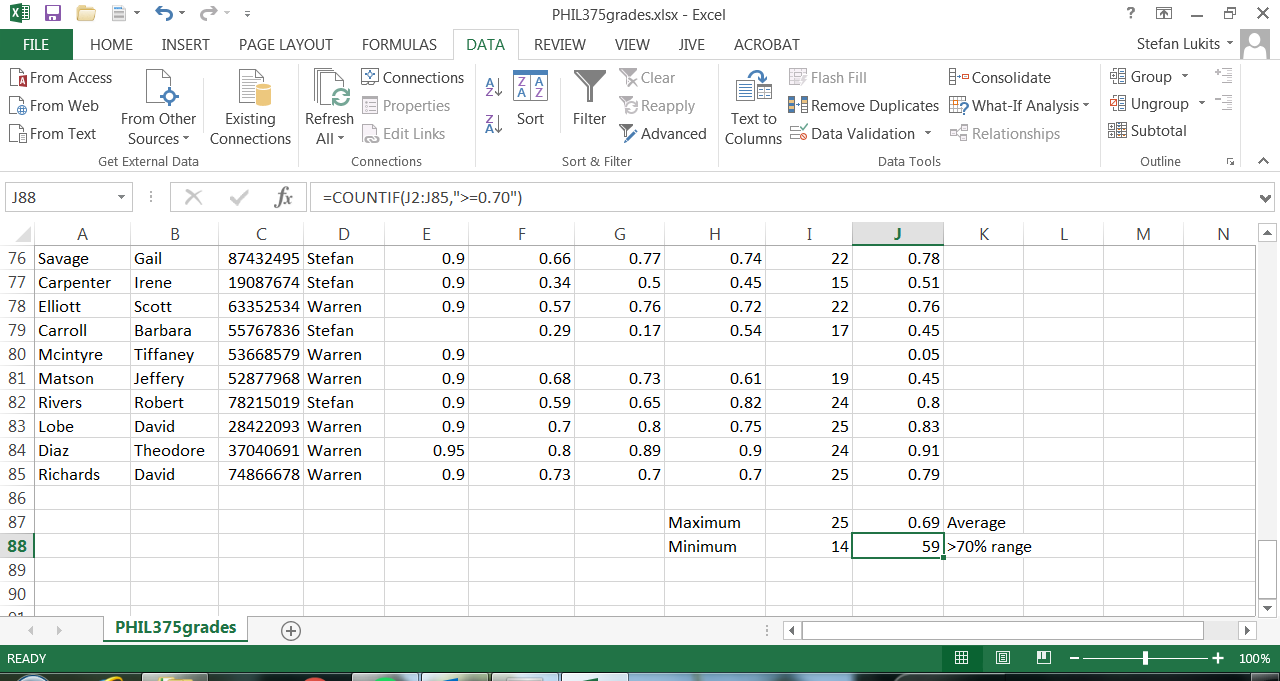
\includegraphics[scale=.42]{./e12.PNG}
  \end{figure}
\end{frame}

\begin{frame}
  \frametitle{PHIL 375 Grades Screen Shot 13}
  \begin{figure}[h]
    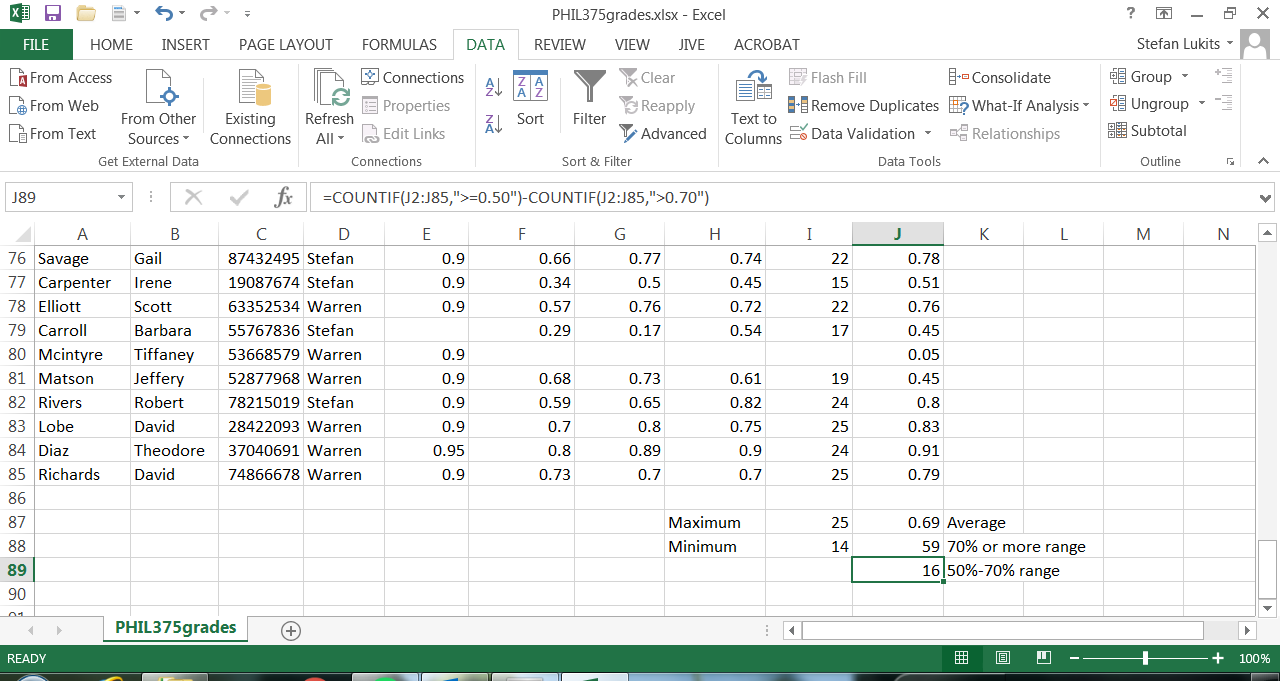
\includegraphics[scale=.42]{./e13.PNG}
  \end{figure}
\end{frame}

\begin{frame}
  \frametitle{PHIL 375 Grades Screen Shot 14}
  \begin{figure}[h]
    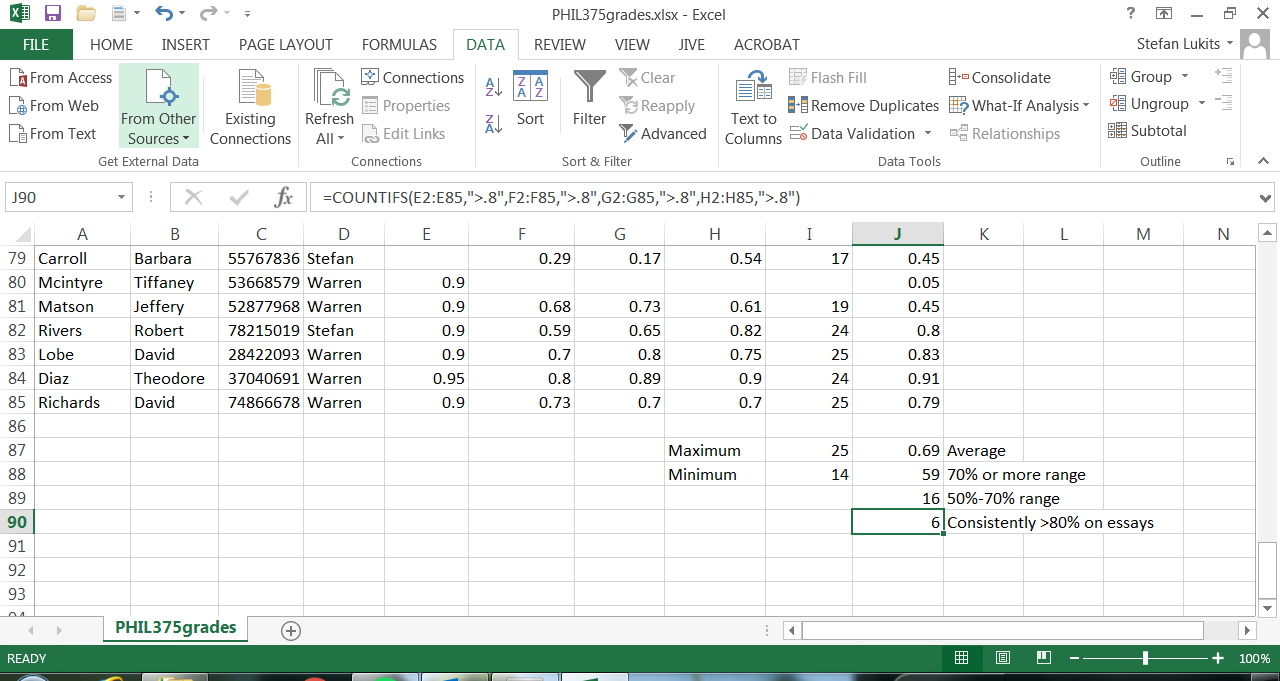
\includegraphics[scale=.42]{./e14.PNG}
  \end{figure}
\end{frame}

\begin{frame}
  \frametitle{End of Lesson}
Next Lesson: Line Fitting
\end{frame}

\end{document}

  % \begin{tabular}{|l|l|}\hline
  %   Excel Function & Description                                                                                             \\ \hline
  %   SUM            & Calculates the sum of a group of values                                                                 \\ \hline
  %   AVERAGE        & Calculates the mean of a group of values                                                                \\ \hline
  %   COUNT          & Counts the number of cells in a range that contains numbers                                             \\ \hline
  %   INT            & Removes the decimal portion of a number leaving just the integer portion                                \\ \hline
  %   ROUND          & Rounds a number to a specified number of decimal places or digit positions                              \\ \hline
  %   IF             & Tests for a true or false condition and then returns one value or another                               \\ \hline
  %   NOW            & Returns the system date and time                                                                        \\ \hline
  %   TODAY          & Returns the system date without the time                                                                \\ \hline
  %   SUMIF          & Calculates a sum from a group of values but just of values that are included because a condition is met \\ \hline
  %   COUNTIF        & Counts the number of cells in a range that match a criteria                                             \\ \hline
  % \end{tabular}
